\documentclass[tikz, margin=3.14mm]{standalone}
\usepackage{pgfplots}
\pgfplotsset{compat=1.18}
\usepgfplotslibrary{statistics}

\usepackage{amsmath, amssymb, amsfonts}

\begin{document}

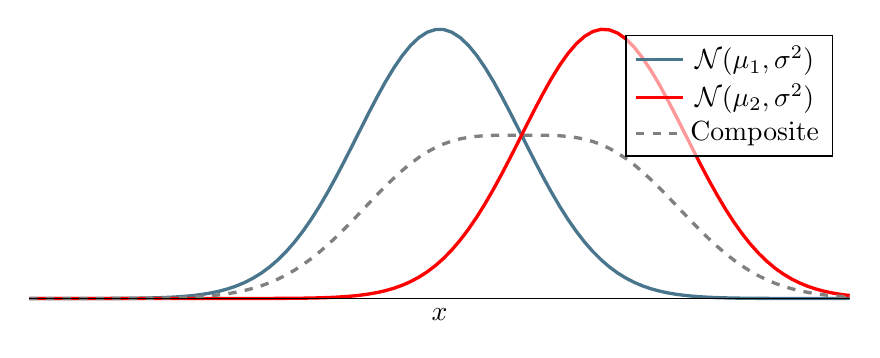
\begin{tikzpicture}
\begin{axis}[
  no markers, 
  domain=0:10, 
  samples=100,
  ymin=0,
  axis lines*=left, 
  xlabel=$x$,
  ylabel=$f(x)$,
  width = 12cm,
  height = 5cm,
  xtick=\empty, 
  ytick=\empty,
  enlargelimits=false, 
  clip=false, 
  axis on top,
  grid = major,
  hide y axis,
  legend style = {fill opacity=0.6, draw opacity=1,text opacity=1},
  ]

  % Men's height distribution
  \addplot [very thick,cyan!50!black] {1/(1*sqrt(2*pi))*exp(-((x-5)^2)/(2*1^2))};
  
  % Women's height distribution
  \addplot [very thick,red] {1/(1*sqrt(2*pi))*exp(-((x-7)^2)/(2*1^2))};
  
  % Composition of both distributions (I'll simply add them up)
  \addplot [very thick,gray,dashed] {.5/(1*sqrt(2*pi))*exp(-((x-5)^2)/(2*1^2)) + .5/(1*sqrt(2*pi))*exp(-((x-7)^2)/(2*1^2))};

  \legend{{$\mathcal N(\mu_1, \sigma^2)$}, {$\mathcal N(\mu_2, \sigma^2)$}, Composite}
\end{axis}
\end{tikzpicture}

\end{document}
